\documentclass{sigchi}

% Use this section to set the ACM copyright statement (e.g. for
% preprints).  Consult the conference website for the camera-ready
% copyright statement.

% Copyright
\CopyrightYear{2020}
%\setcopyright{acmcopyright}
\setcopyright{acmlicensed}
%\setcopyright{rightsretained}
%\setcopyright{usgov}
%\setcopyright{usgovmixed}
%\setcopyright{cagov}
%\setcopyright{cagovmixed}
% DOI
\doi{https://doi.org/10.1145/3313831.XXXXXXX}
% ISBN
\isbn{978-1-4503-6708-0/20/04}
%Conference
\conferenceinfo{CHI'20,}{April  25--30, 2020, Honolulu, HI, USA}
%Price
\acmPrice{\$15.00}

% Use this command to override the default ACM copyright statement
% (e.g. for preprints).  Consult the conference website for the
% camera-ready copyright statement.

%% HOW TO OVERRIDE THE DEFAULT COPYRIGHT STRIP --
%% Please note you need to make sure the copy for your specific
%% license is used here!
% \toappear{
% Permission to make digital or hard copies of all or part of this work
% for personal or classroom use is granted without fee provided that
% copies are not made or distributed for profit or commercial advantage
% and that copies bear this notice and the full citation on the first
% page. Copyrights for components of this work owned by others than ACM
% must be honored. Abstracting with credit is permitted. To copy
% otherwise, or republish, to post on servers or to redistribute to
% lists, requires prior specific permission and/or a fee. Request
% permissions from \href{mailto:Permissions@acm.org}{Permissions@acm.org}. \\
% \emph{CHI '16},  May 07--12, 2016, San Jose, CA, USA \\
% ACM xxx-x-xxxx-xxxx-x/xx/xx\ldots \$15.00 \\
% DOI: \url{http://dx.doi.org/xx.xxxx/xxxxxxx.xxxxxxx}
% }

% Arabic page numbers for submission.  Remove this line to eliminate
% page numbers for the camera ready copy
% \pagenumbering{arabic}

% Load basic packages
\usepackage{balance}       % to better equalize the last page
\usepackage{graphics}      % for EPS, load graphicx instead 
\usepackage[T1]{fontenc}   % for umlauts and other diaeresis
\usepackage{txfonts}
\usepackage{mathptmx}
\usepackage[pdflang={en-US},pdftex]{hyperref}
\usepackage{color}
\usepackage{booktabs}
\usepackage{textcomp}

% Some optional stuff you might like/need.
\usepackage{microtype}        % Improved Tracking and Kerning
% \usepackage[all]{hypcap}    % Fixes bug in hyperref caption linking
\usepackage{ccicons}          % Cite your images correctly!
% \usepackage[utf8]{inputenc} % for a UTF8 editor only

% If you want to use todo notes, marginpars etc. during creation of
% your draft document, you have to enable the "chi_draft" option for
% the document class. To do this, change the very first line to:
% "\documentclass[chi_draft]{sigchi}". You can then place todo notes
% by using the "\todo{...}"  command. Make sure to disable the draft
% option again before submitting your final document.
\usepackage{todonotes}

% Paper metadata (use plain text, for PDF inclusion and later
% re-using, if desired).  Use \emtpyauthor when submitting for review
% so you remain anonymous.
\def\plaintitle{Literature Review}
\def\subplaintitle{
  Reducing Sedentary Behavior for Software Engineers: Identified Performance Advantages and Disadvantages Using a Visual Programming Language Inside Virtual Reality}
\def\plainauthor{First Author, Second Author, Third Author,
  Fourth Author, Fifth Author, Sixth Author}
\def\emptyauthor{}
\def\plainkeywords{Authors' choice; of terms; separated; by
  semicolons; include commas, within terms only; this section is required.}
\def\plaingeneralterms{Documentation, Standardization}

% llt: Define a global style for URLs, rather that the default one
\makeatletter
\def\url@leostyle{%
  \@ifundefined{selectfont}{
    \def\UrlFont{\sf}
  }{
    \def\UrlFont{\small\bf\ttfamily}
  }}
\makeatother
\urlstyle{leo}

% To make various LaTeX processors do the right thing with page size.
\def\pprw{8.5in}
\def\pprh{11in}
\special{papersize=\pprw,\pprh}
\setlength{\paperwidth}{\pprw}
\setlength{\paperheight}{\pprh}
\setlength{\pdfpagewidth}{\pprw}
\setlength{\pdfpageheight}{\pprh}

% Make sure hyperref comes last of your loaded packages, to give it a
% fighting chance of not being over-written, since its job is to
% redefine many LaTeX commands.
\definecolor{linkColor}{RGB}{6,125,233}
\hypersetup{%
  pdftitle={\plaintitle},
% Use \plainauthor for final version.
%  pdfauthor={\plainauthor},
  pdfauthor={\emptyauthor},
  pdfkeywords={\plainkeywords},
  pdfdisplaydoctitle=true, % For Accessibility
  bookmarksnumbered,
  pdfstartview={FitH},
  colorlinks,
  citecolor=black,
  filecolor=black,
  linkcolor=black,
  urlcolor=linkColor,
  breaklinks=true,
  hypertexnames=false
}

% create a shortcut to typeset table headings
% \newcommand\tabhead[1]{\small\textbf{#1}}

% End of preamble. Here it comes the document.
\begin{document}

\title{%
  \plaintitle \\
  \large \subplaintitle
}

\numberofauthors{3}
\author{
  \alignauthor{Adam Jonsson\\
    \affaddr{Stockholm, Sweden}\\
    \email{adajon@kth.se}}\\
}

\maketitle


% ACM Classfication

\begin{CCSXML}
  <ccs2012>
  <concept>
  <concept_id>10003120.10003121</concept_id>
  <concept_desc>Human-centered computing~Human computer interaction (HCI)</concept_desc>
  <concept_significance>500</concept_significance>
  </concept>
  <concept>
  <concept_id>10003120.10003121.10003125.10011752</concept_id>
  <concept_desc>Human-centered computing~Haptic devices</concept_desc>
  <concept_significance>300</concept_significance>
  </concept>
  <concept>
  <concept_id>10003120.10003121.10003122.10003334</concept_id>
  <concept_desc>Human-centered computing~User studies</concept_desc>
  <concept_significance>100</concept_significance>
  </concept>
  </ccs2012>
\end{CCSXML}

\ccsdesc[500]{Human-centered computing~Human computer interaction (HCI)}
\ccsdesc[300]{Human-centered computing~Haptic devices}
\ccsdesc[100]{Human-centered computing~User studies}

\section{Information}
The literature review is divided into different areas thakt can be found as titles in this paper.

\subsubsection{Keywords}
Visual Programming Language, Virtual Reality, Performance, Health.

\section{Sedentary Behavior}

\section{Visual Programming Language}

\section{Virtual Reality}

\subsection{Health}
A potential means of reducing sedentary behavior is using virtual reality (VR) during work. This is because a VR device that uses six degrees of freedom has its benefit in that it requires more movement than being sedentary in front of a computer. A typical VR application might need users to walk, look around, and move their arms to grab or push interactable. Of course, the design of a VR application heavily affects the frequency at which these movements occur. Compare this to a mouse and keyboard setup, where the user only needs to do small movements with their fingers and wrist to interact with a GUI. One meta-analysis on physical training in VR concluded that the technology has potential \cite{ng_effectiveness_2019}

\subsection{Performance}

\subsubsection{Typing}
One issue with VR using hand controllers is the text-input performance. The reason is that current two hand controllers have a limited number of buttons compared to a QWERTY keyboard. As a result, text-input in VR often take use of hand movement, also called select based typing. Marco Speicher et al. explored multiple variation of select base typing and compared the performance to traditional keyboard input \cite{speicher_selection-based_2018}. The multiple select based typing includes: 1) Head pointing, using the head to point at the letter that the user wants to select. 2) Controller pointing, using both controllers to point to letters that the user wants to select. 3) Controller tapping, physically tapping the letters with the controllers. 4) Freehand, using hand tracking were the user is typing on a virtual keyboard. 5) Discrete and continuous cursor, the user uses the buttons on the controller to move a cursor on the keyboard. Their findings was that controller pointing was the most performant in terms of WPM, as well as having the lowest error rate. It was also the most liked by the participants and had the least amount of frustration. However, while controller pointing was the most performant with an average words per minute (WPN) around 15, it falls short compared to keyboard typing with a WPN of 50. It is worth to mention that the study had a fixed distance and size between the user and the virtual keyboard for all different select based typing. Different distances and sizes could therefore potentially give different outcome.

\subsection{User Experience}

\subsubsection{Motion Sickness}
Motion sickness is the phenomenon were the user feel sick after using a VR headset a while. The amount and frequency of motion sickness varies depending on the design of the VR application and the individual resistance to motion sickness. In VR, the cause of motion sickness is mostly due to sensory conflict where movement occur in the virtual world but not in the real physically one \cite{golding_motion_2006}. An example where this can occur is when there is continuous movement by using a joystick to traverse the virtual world without needing to physically move. With six degree of freedom headset, the user can physically move to move in the virtual world, preventing sensory conflict and thus motion sickness. However, limited physically space is one reason why physically movement is not always used to move in the virtual world.


\subsubsection{Accommodation-Vergence Mismatch}
Retinal cues of disparity and blur makes the eyes change accommodation and vergence in order to create one clear image \cite{reichelt_depth_2010}. Accommodation is when the eyes change its focus to create a clear image of what is looked at. If the accommodation fails, the object that is looked at is going to be perceived blurry. Vergence is when the eyes converge or diverge from each other to create a singel image. If vergence fails, visual disparity is perceived, making the object that is looked at appear twice. Accommodation and vergence have been found to be influencing each other, meaning that when accommodation changes, vergence also changes as a reflex, and vice versa \cite{suryakumar_vergence_2007}. Because of this, it is difficult only change accommodation or vergence without changing the other.

In the context of virtual reality headsets, there is a phenomenon called accommodation-vergence mismatch, also called accommodation-vergence conflict \cite{kramida_resolving_2016}. This causes objects to close to the viewer to be blurry or to appear twice. The reson for this is that most VR headsets uses fixed lenses, resulting in a fixed focal length of the viewed content. This means that the user do not need to change their accommodation when using VR. However, the viewer need to alter their vergence due to VR using stereoscopic displays that creates the illusion of 3D. Requiring the viewier to have a fixed accommodation while changing their vergence can cause a accommodation-vergence mismatch, see figure \ref{fig:accommodation_vergence_conflict}. For viewing objects far away, the mismatch is at a level that it is not noticeable for the viewer. However, when object are too close to the headset, the mismatch is at a level that the vision either becomes blurry or have disparity \cite{hoffman_vergenceaccommodation_2008}. This can lead to eye-strain, eye-tiredness and headache \cite{shibata_zone_2011}. For this reason, the viewable content in VR should be placed a a distance such that it minimize accommodation-vergence mismatch.

On study have mapped the viewing distance such that accommodation-vergence mismatch is at a comfortable level \cite{shibata_zone_2011}. They found that discomfort is more promoment when the vergence distance is shorter than the accommodation distance, rather than longer. Looking at figure \ref{fig:comfort_viewing_diagram}, a Oculus Quest 2 headset that has a focal length of 1.3 meter, has a comfortable viewing range about 0.6 meter and more. This is in accordance with the minimum 0.5 meter distance Meta recommends \cite{noauthor_vision_nodate}

\begin{figure}[h]
  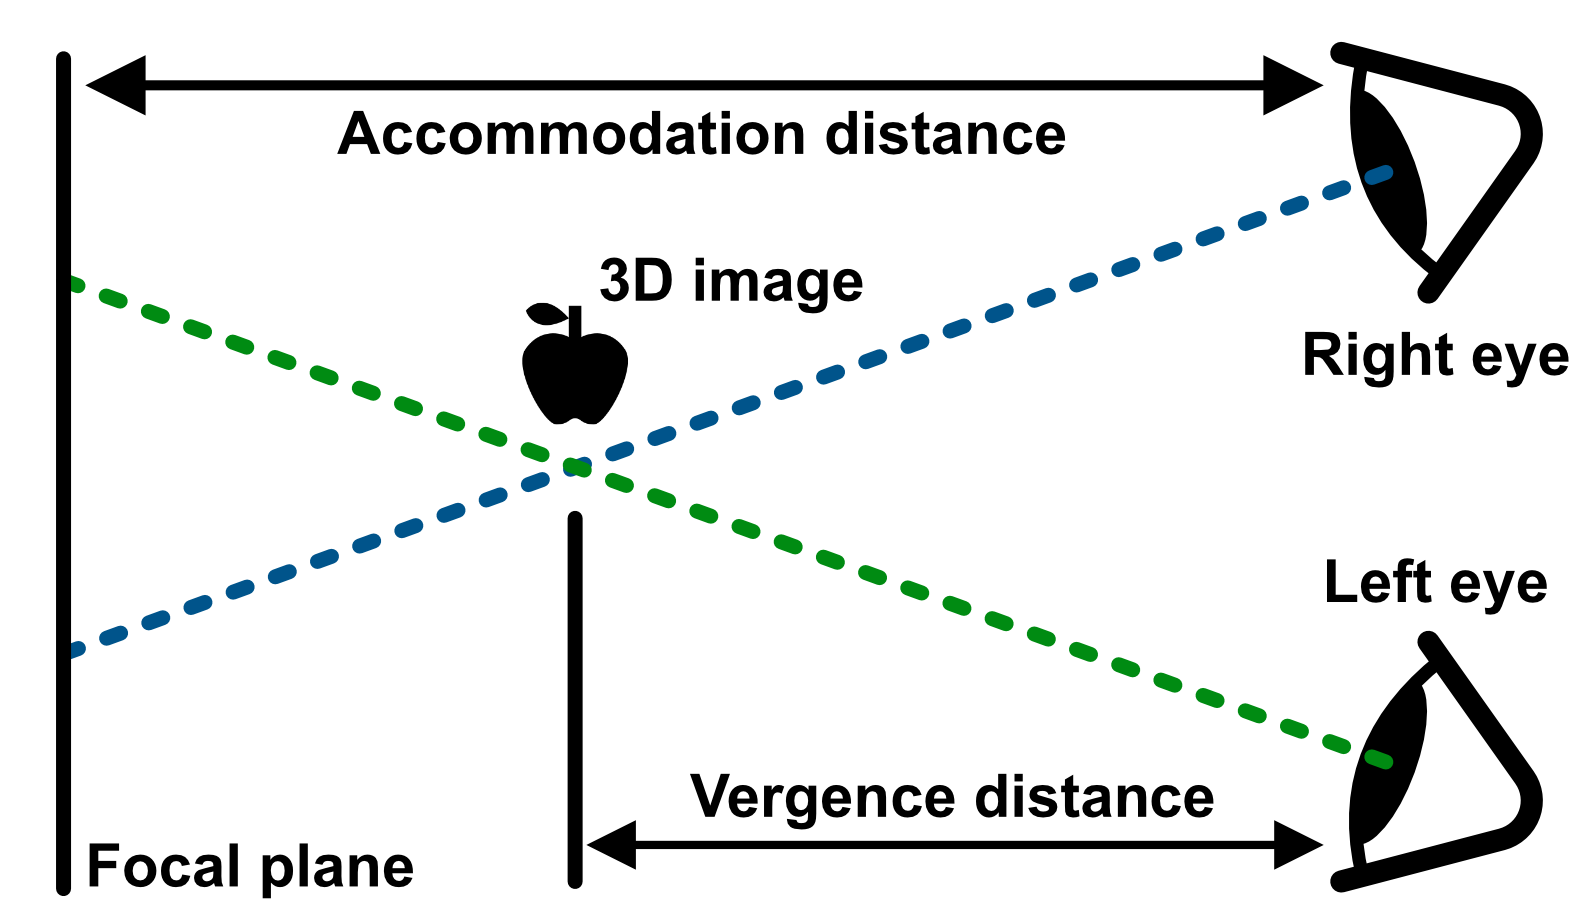
\includegraphics[width=\linewidth]{figures/AccommodationVergenceConflict.png}
  \caption{Example of accommodation and vergence having difference distances, also called accommodation-vergence mismatch}
  \label{fig:accommodation_vergence_conflict}
\end{figure}

\begin{figure}[h]
  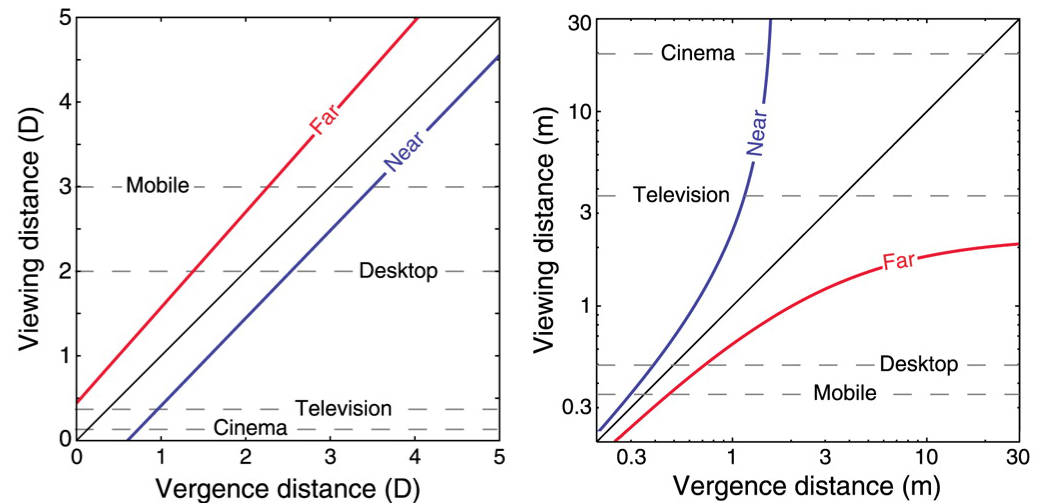
\includegraphics[width=\linewidth]{figures/ComfortViewingDiagram.png}
  \caption{Comfortable viewing distances in terms of accommodation-vergence mismatch}
  \label{fig:comfort_viewing_diagram}
\end{figure}

% Guidelines for the content here: https://scontent.oculuscdn.com/v/t64.5771-25/12482206_237917063479780_486464407014998016_n.pdf?_nc_cat=105&ccb=1-5&_nc_sid=489e6e&_nc_ohc=gGopEQztWKUAX8cS2bj&_nc_ht=scontent.oculuscdn.com&oh=00_AT83tJELVjMHx8T-sZ5NsTAck1iUnVNKXhsy7xQ0VZ7Klg&oe=62133D92

% Source of oculus quest 2 lens focal length https://twitter.com/id_aa_carmack/status/1371485209603022853?lang=se

\section{VPL in VR}
\subsection{Existing VPL designed for VR}

\subsubsection{HackVR}
HackVR is an Object Oriented Programming VPL inside VR. It is design around teaching OOP for new programmings by having challenges that can be solved. It focuses primarily to create a gameification

\subsection{Design}
The size of the blocks is determine on multiple factors. One factor is the screen resolution... Another is the focal length of the lenses, as accomodation-vergence conflict can occure if objects are to close. And third, is the distace which the input system can reach. Using a raycast method allows the user to interact with objects at any distance, but may increase the errors rates such as selecting a block on mistake.

\section{Cognitive Dimensions}
TODO: Explain briefly about what cognitive dimensions are.
% TODO: Read  https://www.researchgate.net/profile/Marian-Petre-4/publication/200085937_Usability_Analysis_of_Visual_Programming_Environments_A_%27Cognitive_Dimensions%27_Framework/links/02bfe50fbf23476730000000/Usability-Analysis-of-Visual-Programming-Environments-A-Cognitive-Dimensions-Framework.pdf

% Form for CD
% http://citeseerx.ist.psu.edu/viewdoc/download?doi=10.1.1.33.7804&rep=rep1&type=pdf

% Papers using Cognitive Dimensions
% https://dl.acm.org/doi/abs/10.1006/ijhc.1994.1029
% http://citeseerx.ist.psu.edu/viewdoc/download?doi=10.1.1.70.5184&rep=rep1&type=pdf

% A different form for evulating CD
% https://d1wqtxts1xzle7.cloudfront.net/45840388/Representation_Design_Benchmarks_a_Desig20160521-17459-1h55j93-libre.pdf?1463866692=&response-content-disposition=inline%3B+filename%3DRepresentation_Design_Benchmarks_A_Desig.pdf&Expires=1647003650&Signature=dZyLVg1~bYZdKIj1M1ldtepBc8jcL1lKQOvfajzRKIB4vOLbx30Esz6~2Oy8B8UG7vK5d~s5~fXHJ8t7pSwFhkl4LEYu9YV71q7asIaPh252skEp4FmY1hcpY4iM9cVW0cpK1xsybRaGJYl3kucLzfSFSvDgb~-OXzN7K8QKgNRcOQ2~H3rMJa78nGF8vPSmiUFsolQwZOKclavRXy-WY1d8PQ996rx~6LefgM~Kd0n1KGmVPcXu3REvakXZMqwBO5MkI0C2BIZvlS94CzDyMg4Fzek4M6KvGYmrKncQzL2ngGvmCTfyy5WJoHElfqX~NC61sn~SdgI3kHSd8B6eBg__&Key-Pair-Id=APKAJLOHF5GGSLRBV4ZA

% TODO: Read about GOMS and argue why we should use it or not use it.
% Seems to be 

One paper by Robert Holwerda and Felienne Hermans explored the potential of using a block based VPL in a professional context. This is in contrast for what block base VPL are usually design for, which is eduction and learnability. The study uses some aspects of cognitive dimensions to evaluated a VPL. The following findings can be of relevance for a VPL in VR.

\subsection{Role-Expressiveness}
\subsubsection{Definition}
% May need to change the example of puzzles pecies
Role-expressiveness is the ability of a program to convey the role or function of a curtain visual element to the user. In Blockly, for example, the blocks are design as puzzles pieces to convey that the blocks are to be connected to each other. Moreover, the shape of the puzzles pieces also give information about what blocks can be connected together.

\subsubsection{Previous findings}
The study by Holwerda and Hermans found two issues with role-expressiveness for their VPL prototype. For one, there was some complaints about the labeling on some of the blocks. Secondly, the participants did not take any use of the comment feature that exited in the VPL. This even after being instructed about the commenting feature. The reasons behind these two issues were not specified in the study. However, some suggested improvements were mentioned. Adding better features for secondary notations were one such suggestion. This could include better commenting, allowing to group blocks, and to add variables and procedures. Having more of these secondary notation would result in better role-expressiveness for the VPL application.

\subsubsection{Potential advantages and disadvantages in VR}
Having a three dimensional environment can potentially contribute to an increased role-expressiveness. For example, comments, labels, or other notation could be shown behind the block it references without obscuring other blocks. The user can then glance behind the block in order to see the different blocks role in the application. However, when the code grows in size, there is a chance that this implementation litter the code space with notation. Making it more confusing instead of increasing role-expressiveness.

\subsection{Role-Expressiveness}

\subsection{???}
One study found that, in terms of role-expressiveness, that screen space was an issue. That block cluster got large enough to

\section{Summary}
\subsection{Design Choices}
\subsubsection{Typing}
Because of the performance issue of using a QWERTY keyboard in VR, design choices that requires text-entry by the user is going to be prevented when possible. However, naming variables, creating strings, and entering numbers are examples where an alternative to text-entry design can be challenging.

\subsubsection{Distance of interactables}
TODO

\section{Evaluation}
\subsection{Motion Sickness}
% Use this for motion sickness:
% https://www.sciencedirect.com/science/article/pii/S000368701730282X?casa_token=jG4Q2R74aCwAAAAA:67n-pb67gF56qdRwBErojiVgAvXPSxzDuSl_bITM2OmosDnqg563SYUGZ2DtkVC5QDiGEe-3Pz4

% REFERENCES FORMAT
% References must be the same font size as other body text.
\bibliographystyle{SIGCHI-Reference-Format}
\bibliography{References}

\end{document}

%%% Local Variables:
%%% mode: latex
%%% TeX-master: t
%%% End:
